\documentclass{article}

\usepackage[tmargin=0.5in,bmargin=0.5in]{geometry}
\usepackage{amsmath, amssymb, amsthm}
\usepackage{listings}
\usepackage{multicol}
\usepackage{enumitem}
\usepackage{forest}
% \usepackage{pdfpages}
\usepackage{graphicx}

\title{CSCI 305 Assignment 3}
\author{(Solo) Isaac Boaz}

\begin{document}
\maketitle

\begin{enumerate}
    \item Provide a \(\Theta\) bound for the solution of each of these recurrences.
          \begin{enumerate}[label=\arabic*.]
              \item \[T(n) = 7T(n/7) + n\]
                    \begin{center}
                        \begin{forest}
                            [$n$
                                [$\frac{n}{7}$
                                        [$\frac{n}{49}$]
                                            [$\frac{n}{49}$]
                                            [$\frac{n}{49}$]
                                            [$\frac{n}{49}$]
                                            [$\frac{n}{49}$]
                                            [$\frac{n}{49}$]
                                            [$\frac{n}{49}$]
                                    ]
                                    [$\frac{n}{7}$
                                        [$\vdots$]
                                    ]
                                    [$\frac{n}{7}$
                                        [$\vdots$]
                                    ]
                                    [$\frac{n}{7}$
                                        [$\vdots$]
                                    ]
                                    [$\frac{n}{7}$
                                        [$\vdots$]]
                                    [$\frac{n}{7}$
                                        [$\vdots$]]
                                    [$\frac{n}{7}$
                                        [$\frac{n}{49}$]
                                            [$\frac{n}{49}$]
                                            [$\frac{n}{49}$]
                                            [$\frac{n}{49}$]
                                            [$\frac{n}{49}$]
                                            [$\frac{n}{49}$]
                                            [$\frac{n}{49}$]
                                    ]
                            ]
                        \end{forest}
                    \end{center}
                    We see each level has \(7^i \cdot \frac{n}{7^i} = n\) work done. Since \(n\) is being divided by \(7\) each level, this will be run \(\log_{7}{n}\) times.
                    \begin{align*}
                        n \cdot \log_7{n} \rightarrow \Theta(n \log n) \\
                    \end{align*}
              \item \[T(n) = 9T(n/3) + n^2\]
                    \begin{center}
                        \begin{forest}
                            [$n^2$
                                [$(\frac{n}{3})^2$
                                        [$(\frac{n}{9})^2$]
                                            [$(\frac{n}{3^2})^2$
                                                [$(\frac{n}{3^3})^2$
                                                        [$\vdots$]
                                                    ]
                                            ]
                                            [$\ddots$]
                                    ]
                                    [$\frac{n^2}{9}$
                                        [$\vdots$]]
                                    [$\frac{n^2}{9}$
                                        [$\vdots$]]
                                    [$\frac{n^2}{9}$
                                        [$\vdots$]]
                                    [$\frac{n^2}{9}$
                                        [$\vdots$]]
                                    [$\frac{n^2}{9}$
                                        [$\vdots$]]
                                    [$\frac{n^2}{9}$
                                        [$\vdots$]]
                                    [$\frac{n^2}{9}$
                                        [$\vdots$]]
                                    [$\frac{n^2}{9}$
                                        [$\vdots$]]
                            ]
                        \end{forest}
                    \end{center}
                    At each level we do \(n^2\) amount of work. Since we're dividing by \(3\) each time, we will do \(\log_3n\) levels.
                    Thus, our runtime is \(n^2 \cdot \log_3 n \rightarrow \Theta(n^2 \log n)\)
              \item \[T(n) = 49T(n/25) + n^{3/2} \log n\]\
                    \begin{multicols}{2}
                        \begin{center}
                            \begin{forest}
                                [$n^{3/2} \log n$
                                    [$49 \times \bigl((\frac{n}{25})^{3/2} \log \frac{n}{25}\bigr)$
                                            [
                                                    $49^2 \times \bigl((\frac{n}{625})^{3/2} \log \frac{n}{625}\bigr)$
                                                    [
                                                            $49^3 \times \bigl((\frac{n}{25^3})^{3/2} \log \frac{n}{25^3}\bigr)$
                                                        ]
                                                ]]
                                ]
                            \end{forest}
                        \end{center}
                        \columnbreak
                        \begin{center}
                            We see that each level does some \(C n^{3/2} \log n\) work. By the definition of \(T(n) = \Theta(f(n))\), \(T(n) = \Theta(n^{3/2})\)
                        \end{center}
                    \end{multicols}
          \end{enumerate}
    \item \pagebreak Draw the recurrence tree for the following recurrence:
          \begin{equation*}
              T(n) = 2T(n/3) + T(3n/4) + c \sqrt{n}
          \end{equation*}
          \begin{center}
              \begin{forest}
                  [$c \sqrt{n}$
                      [$c \sqrt{\frac{n}{3}}$
                              [$c \sqrt{\frac{n}{9}}$]
                                  [$c \sqrt{\frac{n}{9}}$]
                                  [$c \sqrt{\frac{n}{4}}$]
                          ]
                          [$c \sqrt{\frac{n}{3}}$
                              [$c \sqrt{\frac{n}{9}}$]
                                  [$c \sqrt{\frac{n}{9}}$]
                                  [$c \sqrt{\frac{n}{4}}$]
                          ]
                          [$c \sqrt{\frac{3n}{4}}$
                              [$c \sqrt{\frac{n}{4}}$]
                                  [$c \sqrt{\frac{n}{4}}$]
                                  [$c \sqrt{\frac{9n}{16}}$]
                          ]
                  ]
              \end{forest}
              \\
              At level \dots
              \begin{multicols}{2}
                  \begin{enumerate}[label=\arabic*:]
                      \item \(c \sqrt{n}\)
                      \item \(2 c \sqrt{\frac{n}{3}} + c \sqrt{\frac{3n}{4}}\)
                      \item \(4c \sqrt{\frac{n}{9}} + 4c \sqrt{\frac{n}{4}} + c \sqrt{\frac{9n}{16}}\)
                  \end{enumerate}
                  \columnbreak
                  \begin{enumerate}[label=$\rightarrow$]
                      \item \(c \sqrt{n}\)
                      \item \(c( 2\sqrt{\frac{n}{3}} + \sqrt{\frac{3n}{4}})\)
                      \item \(c ( 4(\sqrt{\frac{n}{9}} + \sqrt{\frac{n}{4}}) + \sqrt{\frac{9n}{16}})\)
                  \end{enumerate}
              \end{multicols}

          \end{center}
    \item FFT
          \begin{enumerate}[label=\arabic*.]
              \item Give an asymptotic $\Theta$-bound for lines 1-3.
                    \begin{equation*}
                        \Theta(1)
                    \end{equation*}
              \item Give an asymptotic $\Theta$-bound for lines 6-9.
                    \begin{equation*}
                        \Theta(n)
                    \end{equation*}
              \item What size array is being input and output? \\
                    We see the first array takes the Fourier Transform of the even-indexed elements,
                    and the second array takes the Transform of the odd-indexed elements. Thus, each
                    array is \(n/2\) in size.
              \item Recurrence relation for the cost of \(T(n)\).
                    \begin{align*}
                        T(n) & = 2T(\frac{n}{2}) + O(n) \\
                             & = 2T(\frac{n}{2}) + cn
                    \end{align*}
              \item Solve the above recurrence relation.
                    \begin{center}
                        \begin{forest}
                            [$ cn$
                                [$cn/2$
                                        [$cn/4$]
                                            [$cn/4$]
                                    ]
                                    [$cn/2$
                                        [$cn/4$]
                                            [$cn/4$]
                                    ]
                            ]
                        \end{forest}
                    \end{center}
                    Going by the tree diagram, we see each level \(x\) has \(n\) work.
                    Since we halve the size of the problem each level, there will be \(\log_2n\) levels, amounting to a runtime of
                    \begin{equation*}
                        O(n \log n)
                    \end{equation*}
                    Additionally, since the subtree is balanced, we can say it is both \(O(n \log n)\) and \(\Omega(n \log n)\), and thus \(T(n) = \Theta(n \log n)\).
              \item Find the \(\Theta\) cost of \lstinline|slowFT|.
                    Since the outer \lstinline|for| loop is run \(n\) times, and the inner loop is consequently run \(n^2\) times, we know that \textit{Algorithm 1} is asymptotically faster.
                    \begin{equation*}
                        \Theta(n^2) > \Theta(n \log n)
                    \end{equation*}
          \end{enumerate}
    \item \pagebreak Strass Algorithm
          \begin{enumerate}[label=\arabic*.]
              \item The base case for this algorithm is when it encounters matrices that are \(16 \times 16\) or smaller.
              \item I multiplied a randomly generated 64x64 matrix against another randomly generated 64x64 matrix, the largest
                    squared difference between the two matricies was \(< 1.92 \times 10^{-13}\)
              \item \begin{tabular}{l|c|c}
                        $n$       & $s(n)$  & $m(n)$ \\
                        \hline 32 & 0.0176  & 0.0112 \\
                        64        & 0.0043  & 0.0001 \\
                        128       & 0.0035  & 0.0002 \\
                        256       & 0.0234  & 0.0006 \\
                        512       & 0.1993  & 0.0100 \\
                        1024      & 1.0313  & 0.0150 \\
                        2048      & 7.3894  & 0.1085 \\
                        4096      & 51.6236 & 0.7990
                    \end{tabular}
                    \raisebox{10em}{
                        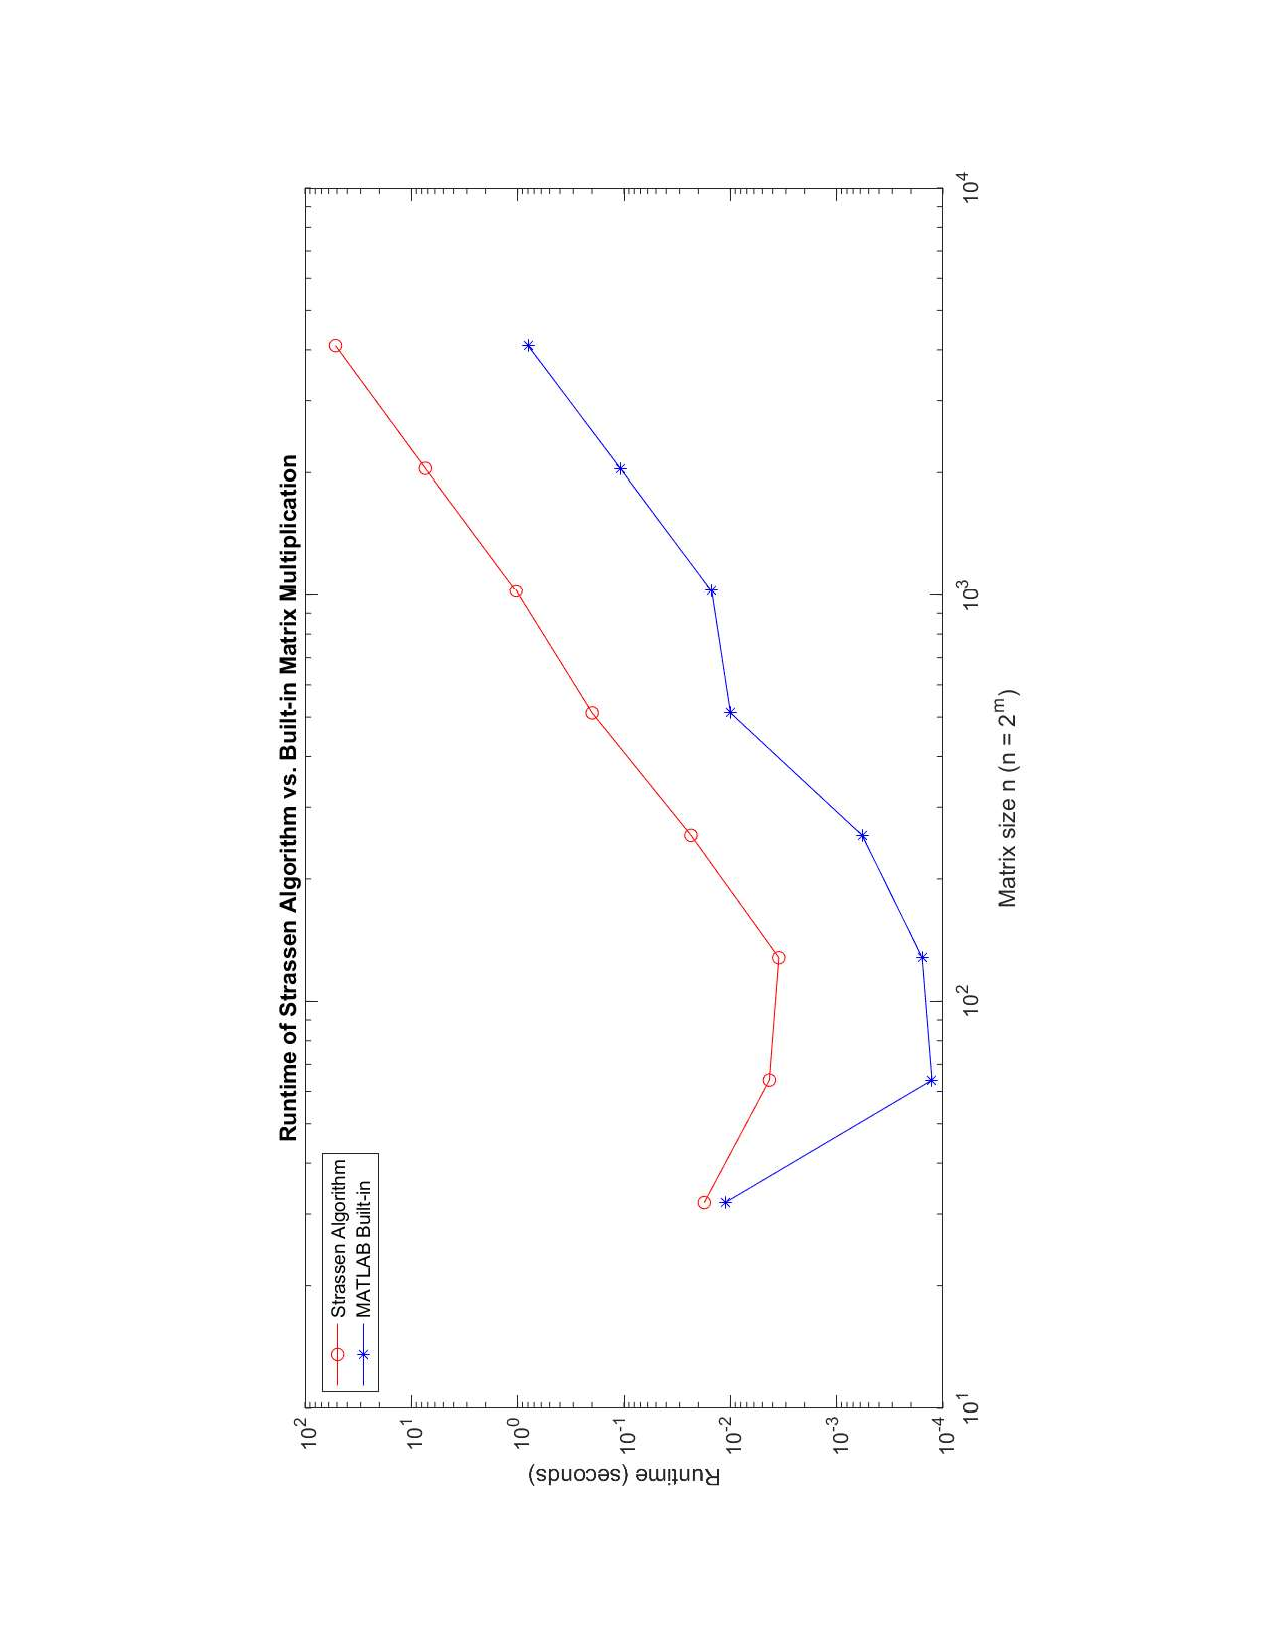
\includegraphics[page=1,angle=270,width=0.7\textwidth]{figure.pdf}
                    }
                    Visually comparing the plot of \(y = x^{\log_27}\) against the original datapoints, it appears the trend lines seems to roughly match, with a constant factor making the Strass algorithm slower.
              \item The naive algorithm for matric multiplication does not do any subtractions, only additions. Strauss' algorithm will only ever do greater than or equal to as many subtractions, making it less stable due to decimal accuracy.
              \item \begin{equation*}
                        T(n) = 7T(\frac{n}{2}) + 6
                    \end{equation*}
          \end{enumerate}

\end{enumerate}


\end{document}